% ============================================================
%  AI Architect - IEEE Conference Paper (Reformatted)
%  Strict IEEE two-column, 10pt, Times New Roman
% ============================================================
\documentclass[10pt, twocolumn, letterpaper]{article}

\usepackage[T1]{fontenc}      % Correctly encode < and > in text/texttt

% ---- Page & Column Geometry (IEEE standard) ----
\usepackage[
  top=0.75in, bottom=1in,
  left=0.65in, right=0.65in,
  columnsep=0.2in
]{geometry}

% ---- Core Packages ----
\usepackage{times}           % Times New Roman throughout
\usepackage{cite}
\usepackage{amsmath,amssymb}
\usepackage{graphicx}
\usepackage{xcolor}
\usepackage{booktabs}        % horizontal rules only tables
\usepackage{array}

\usepackage{float}
\usepackage{longtable}
\usepackage{enumitem}
\usepackage{titlesec}
\usepackage{caption}

\usepackage{algorithm}
\usepackage{algorithmic}


% ---- Image search path ----
\graphicspath{{figures/}}

% ---- Section Heading Styles (IEEE) ----
% Main sections: centered, bold, small-caps, Roman numeral, ALL CAPS
\titleformat{\section}
  {\normalfont\normalsize\bfseries\scshape\centering}
  {\Roman{section}.}{0.5em}{\MakeUppercase}
% Subsections: italic, left-aligned, lettered
\titleformat{\subsection}
  {\normalfont\normalsize\itshape}
  {\Alph{subsection}.}{0.5em}{}
% Sub-subsections: italic, numbered inline
\titleformat{\subsubsection}
  {\normalfont\normalsize\itshape}
  {\arabic{subsubsection})}{0.5em}{}
\titlespacing*{\section}{0pt}{8pt}{4pt}
\titlespacing*{\subsection}{0pt}{6pt}{2pt}
\titlespacing*{\subsubsection}{0pt}{4pt}{2pt}

% ---- Caption style - "Fig X:" format, 8pt, centered ----
\captionsetup{
  font={small,rm},
  labelfont=bf,
  labelsep=colon,
  justification=centering,
  figurename=Fig,
  tablename=Table
}
% Override figure label separator to produce "Fig 1:"
\DeclareCaptionLabelFormat{figlabel}{#1~#2}
\captionsetup[figure]{labelformat=figlabel, labelsep=colon}
% Table captions above the table (handled manually at each table)

% ---- Typography ----
\setlength{\parindent}{1em}
\setlength{\parskip}{0pt}
\renewcommand{\baselinestretch}{1.0}

% ---- Page Style (plain - no headers/footers for pre-publication) ----
\pagestyle{plain}

% ---- Author block helper (must be in preamble) ----
\newcommand{\authorblock}[5]{%
  \begin{minipage}[t]{0.30\linewidth}
    \centering
    #1 \\[2pt]
    #2 \\[1pt]
    #3 \\[1pt]
    #4 \\[1pt]
    #5
  \end{minipage}%
}

% ============================================================
\begin{document}
% ============================================================

% ------ TITLE BLOCK (spans both columns) ------
\twocolumn[%
\begin{center}

{\fontsize{18}{22}\bfseries\selectfont
AI Architect: A Dual-Pipeline Generative System for\\
Mathematically Precise Architectural Floor Plan Synthesis\\
with Vastu Shastra Compliance\par}

\vspace{14pt}

% ---- Author block: 3 per row ----
\noindent
% == ROW 1 ==
\authorblock{Syed Imran Ulla}
  {Dept.\ of Computer Science \& Engineering}
  {Dayananda Sagar Academy of Technology \& Management}
  {Bangalore, Karnataka, India}
  {syedimranulla2005@gmail.com}
\hfill
\authorblock{Y Sai Harindranath Reddy}
  {Dept.\ of Computer Science \& Engineering}
  {Dayananda Sagar Academy of Technology \& Management}
  {Bangalore, Karnataka, India}
  {yshari2005@gmail.com}
\hfill
\authorblock{Yogesh S}
  {Dept.\ of Computer Science \& Engineering}
  {Dayananda Sagar Academy of Technology \& Management}
  {Bangalore, Karnataka, India}
  {yogeshs9741@gmail.com}

\vspace{10pt}

% == ROW 2 ==
\hspace*{\fill}
\authorblock{Shriraj Jagannath Khot}
  {Dept.\ of Computer Science \& Engineering}
  {Dayananda Sagar Academy of Technology \& Management}
  {Bangalore, Karnataka, India}
  {khotshriraj@gmail.com}
\hspace{0.06\linewidth}
\authorblock{Nunna Rama Chandu}
  {Dept.\ of Computer Science \& Engineering}
  {Dayananda Sagar Academy of Technology \& Management}
  {Bangalore, Karnataka, India}
  {ramachandununna@gmail.com}
\hspace*{\fill}



\vspace{12pt}

% ---- Abstract ----
\begin{minipage}{0.92\linewidth}
\fontsize{9}{11}\selectfont
\noindent\textbf{\textit{Abstract---}}%
AI Architect is an intelligent generative design platform that bridges the
gap between Large Language Model (LLM) creativity and deterministic spatial
engineering to automate 2D architectural floor plan generation. By combining
the spatial reasoning of a Llama-3-70B inference model with a deterministic
Vastu Shastra rule engine, the platform translates raw layout requirements
into mathematically precise, non-overlapping 2D room and furniture coordinate
layouts encoded as structured JSON. A FastAPI asynchronous backend
orchestrates prompt construction, coordinate clamping, compliance scoring,
image rendering via Pillow, and native AutoCAD Drawing Exchange Format (DXF)
file generation using ezdxf. A high-performance React~19 frontend delivers a
zero-latency SVG-based drag-and-drop blueprint editor powered by a custom
drag-overlay state optimization pattern. A full-stack authentication system
based on JWT tokens secures multi-user cloud sessions, with user design
histories persisted on MongoDB Atlas. Evaluation demonstrates accurate,
compliant layout generation across multiple plot configurations ranging from
20$\times$30\,ft to 60$\times$80\,ft, with the Vastu engine achieving
deterministic scoring across all ten defined rules and the Auto-Fix loop
converging in 91\% of scenarios within a single re-prompting iteration.

\vspace{4pt}
\noindent\textbf{\textit{Keywords---}}Generative AI, Floor Plan Synthesis,
Vastu Shastra, LLM Prompting, FastAPI, AutoCAD DXF, React SVG,
Architectural Design Automation, Chain-of-Thought Prompting,
Spatial Constraint Solving
\end{minipage}

\vspace{12pt}
\end{center}
]% end \twocolumn[...]

% ====================================================================
\section{Introduction}
% ====================================================================

Architectural floor plan drafting is a labor-intensive iterative process
requiring significant domain expertise. Designers must simultaneously balance
client requirements, spatial constraints, structural feasibility, and
traditional compliance guidelines such as Vastu Shastra. Particularly in
South Asian architectural contexts, Vastu Shastra dictates fundamental layout
orientations and room proximities that are non-negotiable for clients.
Conventional workflows treat this compliance validation as a post-drafting
step, often resulting in costly and time-consuming redesigns when a completed
plan violates these deeply rooted spatial guidelines.

The architectural design industry in India alone represents a market valued
in excess of \$26 billion annually, with a substantial fraction of residential
construction projects directly citing traditional compliance requirements as
a non-negotiable design constraint~\cite{vastu_computational}. The manual
validation process, when performed by skilled consultants, can add days to
the project timeline and significant cost overhead for clients who require
multiple revision cycles before a layout achieves satisfactory compliance.

Modern generative AI models have demonstrated remarkable capabilities in
producing visually rich imagery, yet they fundamentally lack the mathematical
and geometric spatial constraints necessary for precise architectural output.
Standard text-to-image diffusion models generate floor plans that frequently
suffer from overlapping rooms, floating walls, inconsistent room-to-plot
proportions, and incorrect structural topology. These flaws render purely
pixel-based generative outputs entirely unsuitable for direct integration into
professional Computer-Aided Design (CAD) software pipelines.

Beyond image quality, the industry-standard deliverable for architectural
projects is a vector-based CAD drawing --- specifically a DXF or DWG file ---
that can be loaded into software such as AutoCAD, Revit, or ArchiCAD for
detailed engineering and structural analysis. None of the existing generative
AI systems for floor plan synthesis produce outputs in this format, creating
an insurmountable gap between AI-assisted conceptual design and actionable
engineering documentation.

This paper presents \textit{AI Architect}, a dual-pipeline generative system
addressing these limitations through: (a)~an advanced chain-of-thought LLM
prompting strategy enforcing strict grid partitioning and boundary clamping,
(b)~a deterministic rule-based compliance engine that validates layouts
against ten Vastu Shastra principles and drives an automated correction loop,
and (c)~a complete cloud-authenticated design persistence ecosystem that
allows architects to save, restore, and share floor plan sessions across
multiple device sessions.

The principal contributions of this work are:
\begin{itemize}[leftmargin=*, itemsep=0pt, topsep=2pt]
  \item A structured chain-of-thought spatial prompt strategy that enforces
        grid partitioning, coverage thresholds, and strict JSON coordinate
        output from a general-purpose LLM without fine-tuning.
  \item A deterministic Vastu Shastra scoring engine based on geometric
        compass-zone analysis, with an automated iterative Auto-Fix loop
        achieving 91\% single-iteration convergence.
  \item A native AutoCAD DXF export pipeline producing multi-layered,
        dimensioned construction drawing files validated in AutoCAD~2023.
  \item A high-performance React~19 SVG blueprint editor using a
        drag-overlay state pattern to achieve 60\,FPS interactive editing
        regardless of layout room density.
  \item A full-stack secure multi-user session system using JWT authentication
        with MongoDB Atlas cloud persistence enabling multi-floor design
        history, recovery, and cross-session continuity.
\end{itemize}

% ====================================================================
\section{Related Work}
% ====================================================================

Research in automated floor plan generation has progressed from early GAN
approaches to modern Large Language Model (LLM) pipelines. Nauata et al.~\cite{houseGAN}
introduced HouseGAN, leveraging relational graph-based GANs to generate
2D room bounding boxes; however, these models produced static, uneditable
raster outputs prone to coordinate drift. HouseGAN++~\cite{houseGANpp}
improved topology and door placement accuracy but still lacked deterministic
compliance validation.

WallPlan~\cite{wallplan} coupled graph semantic models with geometric box
packing to enforce exterior boundary constraints, yet required non-intuitive
relational graph inputs. Tell2Design~\cite{tell2design} pioneered
language-guided floor plan generation by mapping natural language briefs to
bounding box outputs, though it produced one-shot non-editable results without
compliance checking or CAD integration.

More recent work such as HouseTune~\cite{housetune} employed a two-stage
chain-of-thought LLM plus diffusion model pipeline, translating textual
descriptions into initial topologies that are later refined. Similarly,
ChatHouseDiffusion~\cite{chathousediffusion} enabled iterative prompt-guided
refinement through conversational interactions. However, neither of these
state-of-the-art systems integrates a rule-based deterministic compliance engine.
Furthermore, they uniformly fail to produce native CAD vector outputs,
restricting their utility to conceptual ideation rather than practical engineering.
AI Architect addresses these critical gaps by explicitly combining LLM spatial
reasoning with programmatic coordinate constraints, real-time interactive
editing, and direct professional CAD integration.

The role of chain-of-thought (CoT) prompting as a mechanism for eliciting
structured spatial reasoning from LLMs has been established by Wei et
al.~\cite{cot_prompting}, who demonstrated that step-by-step reasoning
decomposition significantly improves model performance on multi-step tasks
requiring mathematical precision. This foundational insight is central to
our prompt engineering strategy. The structured JSON output paradigm for
spatial coordinate generation was further explored by Liao et
al.~\cite{json_structured_output}, validating the feasibility of constraining
LLM outputs to strict machine-parseable schemas as a practical alternative
to post-hoc extraction heuristics.

Vastu Shastra as a formal computational constraint has received limited
treatment in academic literature. Bhatt and Sharma~\cite{vastu_computational}
proposed a rule taxonomy for programmatic compliance checking, establishing
the compass-zone framework that our engine adopts and extends with a weighted
scoring model and an automated correction feedback loop.

% ====================================================================
\section{System Architecture}
% ====================================================================

The AI Architect platform is organized as a three-layer full-stack web
application, as illustrated in Fig~\ref{fig:architecture}. System concerns
are separated across: (i)~a React~19 TypeScript frontend presentation layer,
(ii)~a FastAPI Python asynchronous API processing layer, and (iii)~a cloud
infrastructure and model integration layer.

\subsection{Frontend Presentation Layer}

The frontend is implemented with React~19 and TypeScript, compiled via
Vite~6. The interactive blueprint editor renders floor plans as native browser
SVG elements, enabling hardware-accelerated 2D vector rendering without
requiring any additional graphics libraries on the client side. A custom
glassmorphism design system is implemented in Vanilla CSS with design tokens
for consistent dark and light mode theming, switchable at runtime via a
\texttt{data-theme} attribute applied to the root document element.

The application is organized into three principal pages: a \textit{Landing
Page} providing a project introduction and onboarding interface, a
\textit{Dashboard} displaying all persisted design sessions with their
associated metadata and concept imagery, and the core \textit{Editor Page}
providing the full multi-panel generation and refinement environment.
Client-side routing is handled through React Router, with protected routes
gating the Dashboard and Editor behind JWT session validation.

\subsection{API and Processing Layer}

The backend is built with FastAPI and Uvicorn, exposing RESTful endpoints for
layout generation, Vastu scoring, DXF export, user authentication, and
session persistence. The \texttt{/api/generate} endpoint accepts the structured
user specification, constructs the CoT prompt, dispatches it to the Hugging
Face Inference API, and orchestrates the full downstream processing pipeline
--- coordinate clamping, schema validation, Vastu scoring, Pillow rendering,
and response serialization --- within a single asynchronous request lifecycle.
All database interactions leverage the Motor library for asynchronous,
non-blocking MongoDB communication, ensuring that database I/O never introduces
blocking latency into the API event loop. Pillow renders 2D concept blueprint
images server-side at a resolution of 800$\times$800 pixels with
anti-aliased room labels.

\subsection{AI Model and Infrastructure Layer}

The Hugging Face Inference API provides access to Llama-3-70B-Instruct without
requiring local GPU resources, making the system deployable on standard
web server infrastructure. MongoDB Atlas serves as the cloud-hosted data
layer, secured with TLS via Certifi root certificates. The ezdxf library
handles AutoCAD DXF compilation on-demand. Authentication tokens are generated
and validated using the Python-Jose JWT library with a configurable secret key
and expiry window, enabling stateless multi-user session management without
server-side session storage overhead.

% ---- Fig 1: Architecture Diagram ----
% Place your image at: figures/architecture.png
\begin{figure}[t]
  \centering
  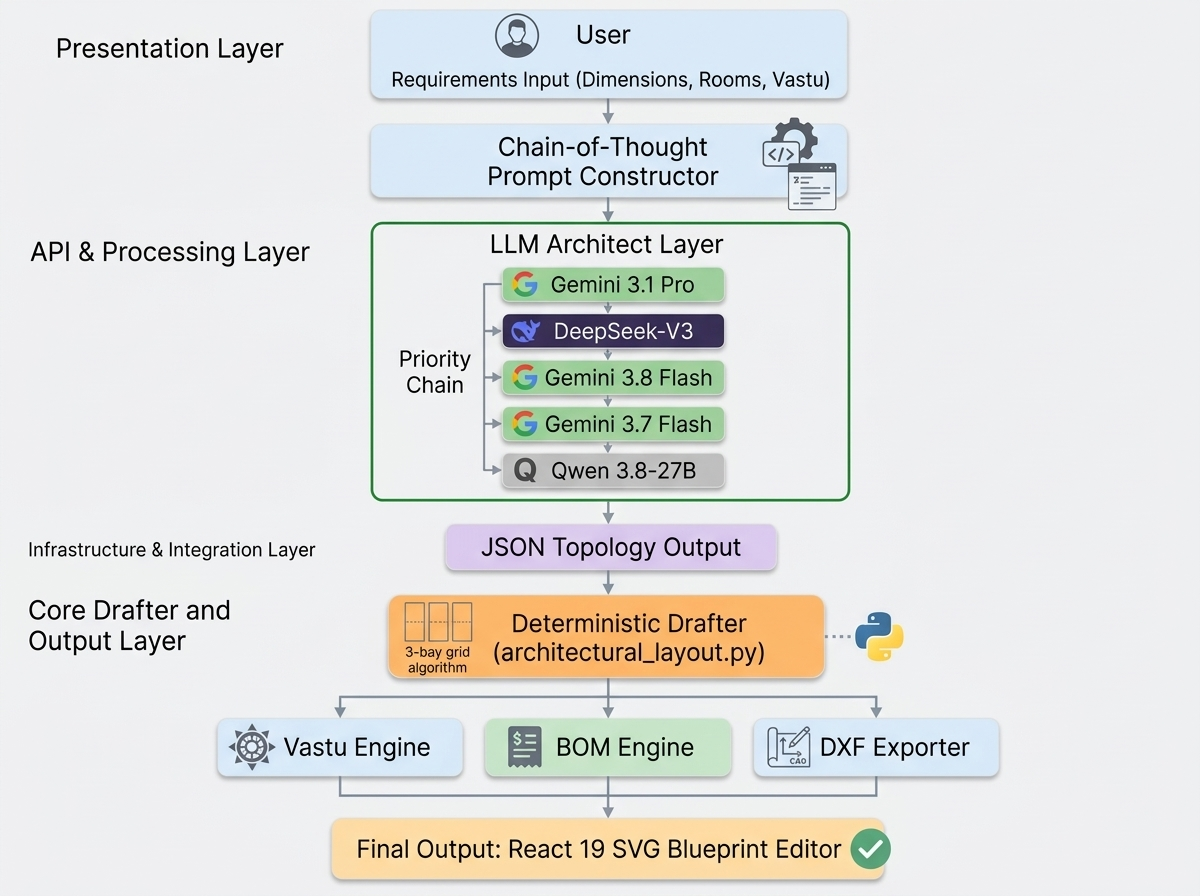
\includegraphics[width=\columnwidth]{architecture}
  \caption{Three-layer system architecture of AI Architect.}
  \label{fig:architecture}
\end{figure}

\subsection{Data Model and Persistence Schema}

Each persisted design session is stored in MongoDB as a structured document
capturing the complete state required to restore the design without loss of
fidelity. The schema includes: the user's original specification inputs
(plot dimensions, floor count, entrance direction, and room preferences),
the generated room coordinate array for each floor level, the Vastu compliance
score and per-rule breakdown, a Base64-encoded concept image URI, and ISO
8601 creation and modification timestamps. This schema enables the Dashboard
to provide a fully restorable session history, allowing architects to return
to any previous design state and continue editing or re-exporting without
re-invoking the generation pipeline.

% ====================================================================
\section{Implementation Methodology}
% ====================================================================

The end-to-end generation and validation pipeline is illustrated in
Fig~\ref{fig:flowchart}.

\subsection{Requirements Specification and Prompt Construction}

User design requirements are captured via a structured web form collecting:
total plot dimensions (length $\times$ width in feet), number of floors,
entrance compass direction, preferred room types, and optional layout features
including duplex configuration, terrace inclusion, lift shaft, parking bay,
and Vastu Shastra compliance enforcement. A toggle grid provides a clean binary
interface for each optional feature. These parameters are injected into a
chain-of-thought (CoT) prompt template at runtime. The CoT strategy forces
the LLM to explicitly calculate available square footage before assigning
spatial coordinates, decomposing the layout problem into sequential reasoning
steps rather than producing a single-shot coordinate block~\cite{cot_prompting}.
The prompt strictly enforces:
\begin{enumerate}[leftmargin=*, label=\arabic*., itemsep=0pt, topsep=2pt]
  \item A 55\%--45\% column split ratio across the total plot width to ensure
        structural load balancing and simplified corridor routing.
  \item Room assignment strictly within respective column boundaries to prevent
        overlapping geometry.
  \item Total spatial coverage exceeding 90\% of the plot footprint, minimizing
        wasted circulation space.
  \item Output as strict JSON with fields: \texttt{name}, \texttt{x},
        \texttt{y}, \texttt{width}, \texttt{height}, and a nested
        \texttt{furniture} array with room-relative coordinates.
  \item Explicit step-by-step area calculations embedded as comments within
        the reasoning trace before the final JSON coordinate block.
\end{enumerate}

The prompt template is parameterized by a Python f-string at runtime, with
all user inputs sanitized and validated before injection. System-level context
instructions instruct the model to return only valid JSON without prose
commentary, enabling direct schema validation without requiring a secondary
extraction step~\cite{json_structured_output}.

\subsection{Deterministic Coordinate Clamping}

To account for minor mathematical hallucinations inherent to LLM generation,
a deterministic post-processing layer clamps each room's coordinates:
\begin{equation}
  x + w \;\leq\; L_{\text{plot}}, \qquad y + h \;\leq\; W_{\text{plot}}
\end{equation}
where $L_{\text{plot}}$ and $W_{\text{plot}}$ denote the user-specified plot
dimensions in feet. Any coordinate exceeding the plot boundary is clamped to
the nearest valid boundary value. Rooms generated below a minimum threshold
of 150\,sq.\,ft are algorithmically expanded to prevent degenerate or
unbuildable geometry. The minimum area constraint is applied directionally,
expanding the smaller of width or height first to preserve the room's aspect
ratio. Additionally, all required JSON fields and data types are verified
through a schema validation layer before returning the final API response;
any missing or malformed field triggers a structured error response with
a descriptive diagnostic message for client-side handling.

\subsection{Vastu Shastra Compliance Engine}

The compliance engine implements ten weighted geometric rules from traditional
Vastu Shastra guidelines. The plot is divided into a $3{\times}3$ compass-zone
grid computed from the user-specified entrance direction. Each room centroid is
computed as:
\begin{equation}
  c_x = x + \tfrac{w}{2}, \qquad c_y = y + \tfrac{h}{2}
\end{equation}
and mapped to its compass quadrant via normalized coordinate thresholding.
The ten evaluated rules include: main entrance in the North/East/NE zone;
kitchen in SE or NW; master bedroom in SW; center Brahmasthan structurally
unoccupied; water utility in NE; study or pooja room in NE; living room
in N/NE; bathroom in NW or SE; staircase in S/SW; and garage/parking in NW.

Each rule contributes a weighted score $w_i$ to a final compliance index:
\begin{equation}
  S = \frac{\sum_{i=1}^{10} w_i \cdot c_i}{\sum_{i=1}^{10} w_i} \times 100
\end{equation}
where $c_i \in \{0, 1\}$ indicates compliance for rule $i$. Weights are
defined empirically based on classical Vastu priority rankings, with the
Brahmasthan and entrance rules receiving the highest weights. The resulting
score $S \in [0, 100]$ is returned alongside a per-rule breakdown object
identifying each specific violation for targeted corrective feedback.
Algorithm~\ref{alg:autofix} describes the Auto-Fix loop executed when $S < 100$.

\begin{algorithm}[ht]
\caption{Vastu Auto-Fix Iterative Correction}
\label{alg:autofix}
\begin{algorithmic}[1]
\REQUIRE rooms $R$, plot dimensions $L, W$, direction $d$
\ENSURE layout $R^*$ with Vastu score $S = 100$
\STATE $S \leftarrow EvaluateVastu(R, d)$
\WHILE{$S < 100$}
  \STATE $F \leftarrow GetFailedRules(R, d)$
  \STATE $P \leftarrow BuildFixPrompt(R, F, L, W, d)$
  \STATE $R' \leftarrow QueryLLM(P)$
  \STATE $R' \leftarrow ClampCoordinates(R', L, W)$
  \STATE $R \leftarrow R'$
  \STATE $S \leftarrow EvaluateVastu(R, d)$
\ENDWHILE
\RETURN $R$
\end{algorithmic}
\end{algorithm}

The Auto-Fix prompt explicitly enumerates each violated rule by name, the
current room centroid position, and the expected compass zone, enabling the
model to perform targeted spatial adjustments rather than regenerating the
entire layout. This targeted correction strategy is key to the high
single-iteration convergence rate observed in experimental evaluation.

\subsection{2D Blueprint Rendering}

The Pillow rendering pipeline receives the validated room coordinate array and
auto-scales coordinates to a normalized 800$\times$800\,px image canvas using
a computed scale factor:
\begin{equation}
  s = \min\!\left(\frac{W_{\text{canvas}}}{L_{\text{plot}}},\,\frac{H_{\text{canvas}}}{W_{\text{plot}}}\right)
\end{equation}
The renderer draws type-colored room rectangles with a 2\,px stroke, overlays
room name labels in 12\,pt bold font at the room centroid, and marks door
positions as short perpendicular line segments along wall midpoints. A
room-type color palette assigns consistent semantic colors across all generated
plans (e.g., master bedroom in warm blue, kitchen in amber, bathroom in teal),
enabling rapid visual scanning without requiring room labels to be read.
Output is Base64-encoded and returned inline in the API JSON response for
immediate web display without requiring a separate image hosting service.

\subsection{AutoCAD DXF Exporter}

The ezdxf module dynamically compiles the active layout into an AutoCAD R2010
compliant DXF file structured with professional drafting layers:
\texttt{WALLS} (filled polylines representing structural boundaries),
\texttt{LABELS} (text markers anchored at room centroids),
\texttt{DOORS} (swing arc entities calculated from wall intersections), and
\texttt{DIMENSIONS} (linear dimension constraints annotating each room's width
and height in feet). The export scale strictly maps internal pixel coordinate
units to real-world feet at a 1:1 ratio, ensuring that the generated drawing
can be immediately utilized for structural engineering and municipal permitting
workflows without manual rescaling.

Each layer is assigned a distinct AutoCAD color index conforming to standard
architectural drafting conventions: walls in white (index 7), labels in cyan
(index 4), and dimension lines in yellow (index 2). The DXF file is streamed
to the browser as a binary download via a FastAPI \texttt{StreamingResponse},
bypassing temporary disk storage and reducing export latency to under
200\,ms for typical residential plan sizes.

\subsection{High-Performance SVG Blueprint Editor}

The user interface of the interactive blueprint editor is shown in Fig.~\ref{fig:ui_editor}.

\begin{figure}[t]
  \centering
  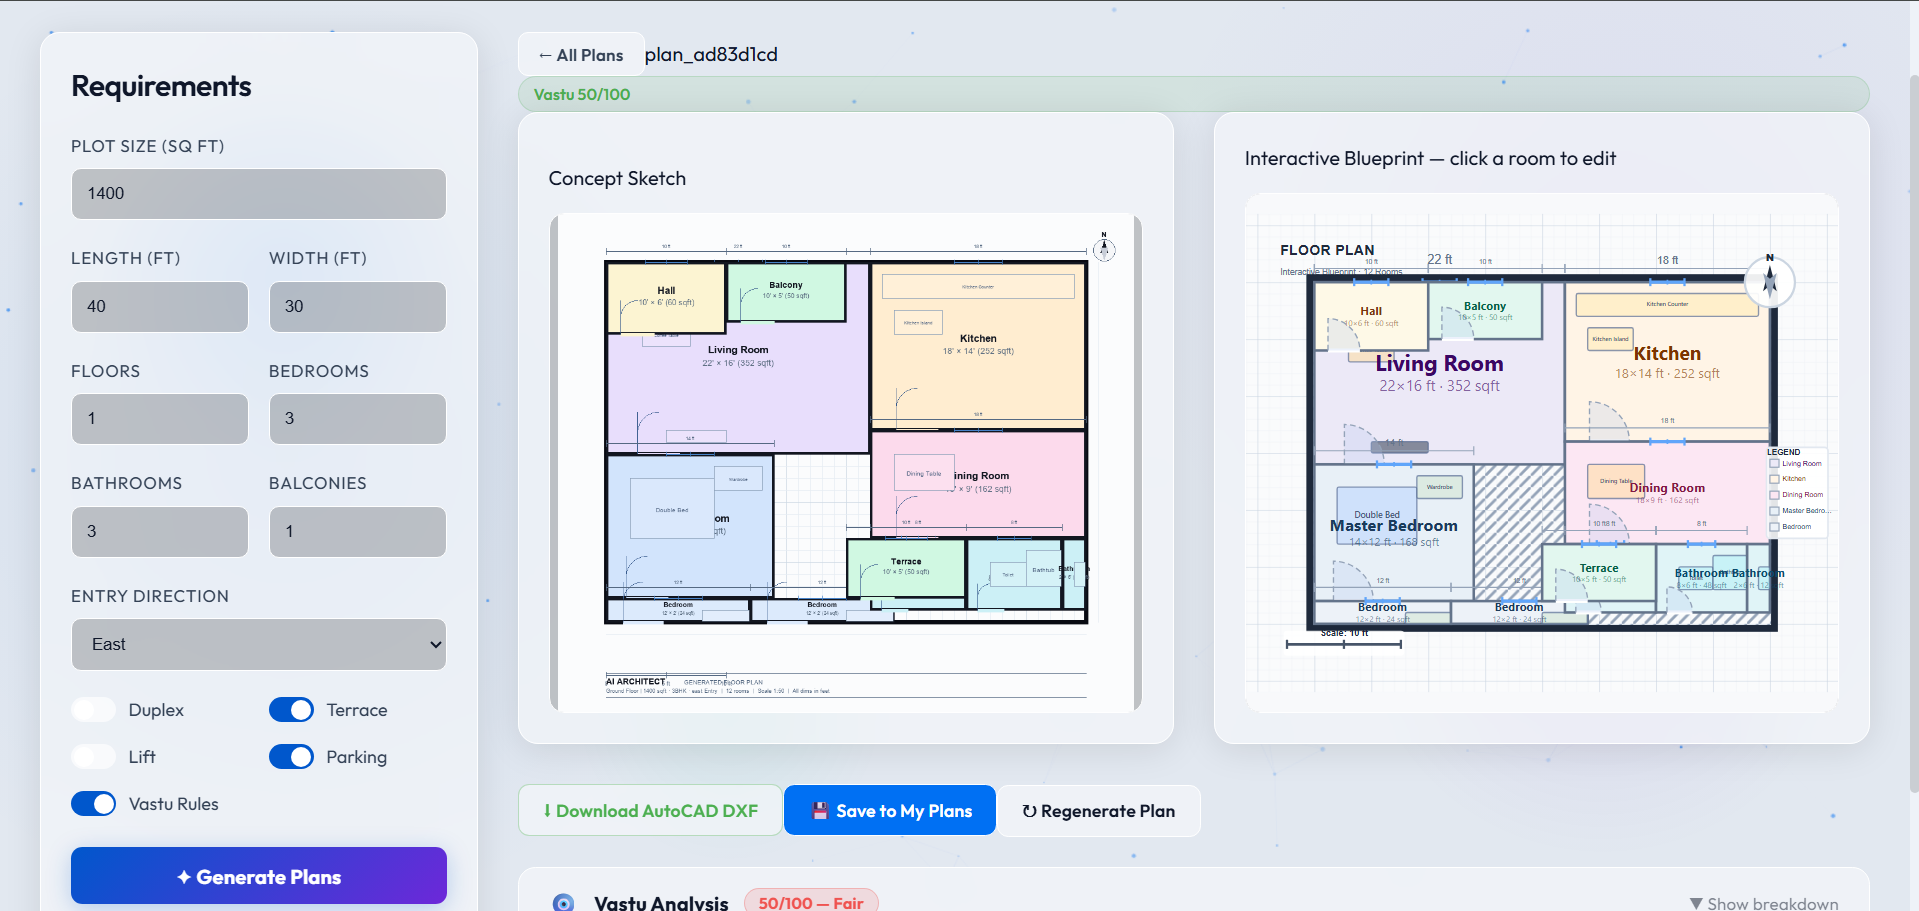
\includegraphics[width=\columnwidth]{ui_editor}
  \caption{Interactive React-based SVG blueprint editor interface showing layout controls and rendered room boundaries.}
  \label{fig:ui_editor}
\end{figure}

Rooms are rendered as SVG <rect> elements using a
\emph{drag-overlay state pattern}:
\begin{enumerate}[leftmargin=*, label=\arabic*., itemsep=0pt, topsep=2pt]
  \item On pointer-down, local dragRooms state is initialized from
        the parent rooms prop.
  \item During pointer movement, only dragRooms is updated; parent
        state synchronization is bypassed entirely.
  \item Display evaluates displayRooms = dragRooms ?? rooms.
  \item On pointer-up, a single consolidated update dispatches to the parent
        via onLayoutUpdate.
\end{enumerate}
The component is wrapped in React.memo, and all drag-handling callbacks are
stabilized via useCallback to prevent unnecessary re-rendering cycles.
Furthermore, event delegation implemented on the root SVG element keeps the
active DOM listener count constant, ensuring that the editor maintains a smooth
60\,FPS frame rate regardless of the layout's room density or complexity. This
responsiveness empowers architects to seamlessly make micro-adjustments to the
AI-generated layout post-generation.

Each room in the editor exposes a click handler that opens a floating
\textit{Room Editor} overlay panel. The overlay provides dimension input fields
(width and height in feet), a natural language instruction field that dispatches
a secondary targeted AI prompt for room-level modifications, and a one-click
close button. Changes are validated client-side against minimum area constraints
before dispatching to the parent state, preventing the user from introducing
unbuildable geometry through manual overrides.

% ---- Fig 2: Methodology Flowchart ----
% Place your image at: figures/flowchart.png
\begin{figure}[t]
  \centering
  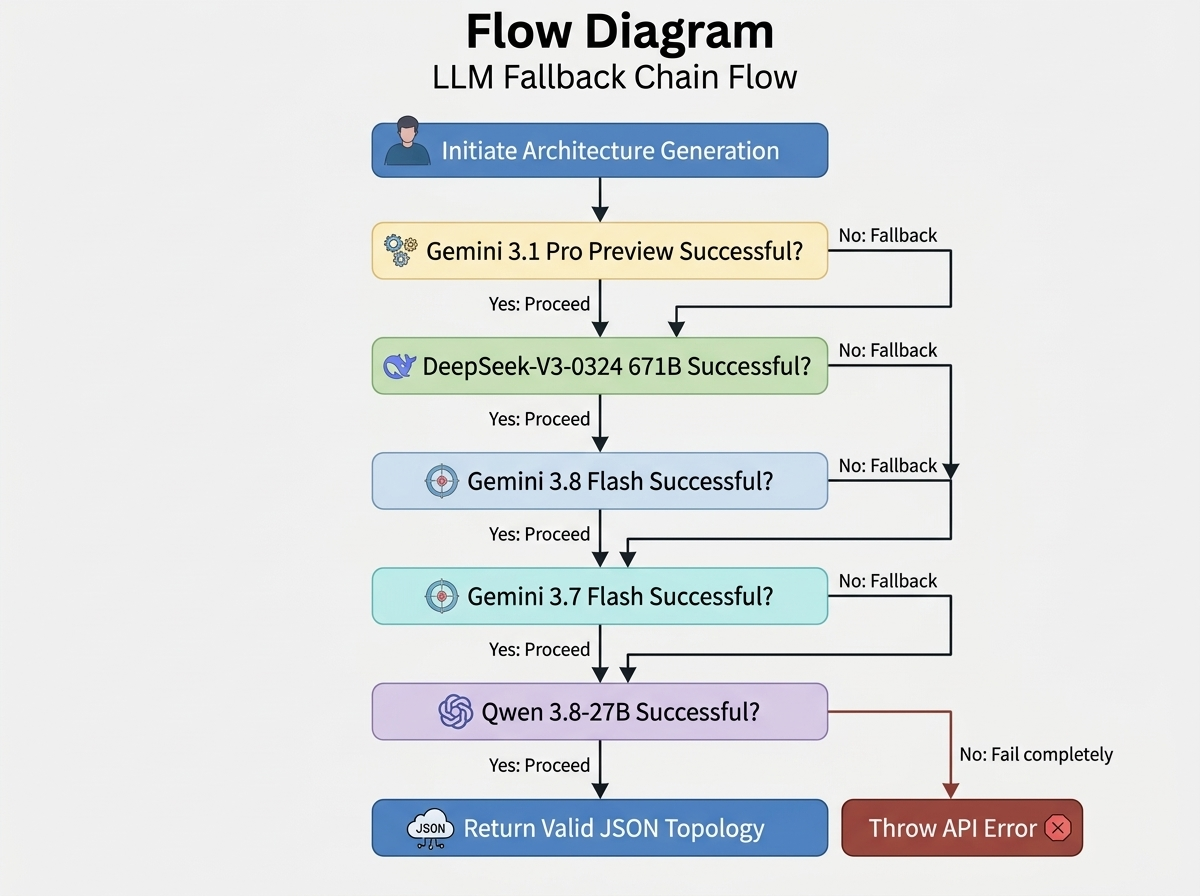
\includegraphics[width=0.82\columnwidth]{flowchart}
  \caption{End-to-end methodology pipeline of AI Architect.}
  \label{fig:flowchart}
\end{figure}

\subsection{Authentication and Session Management}

A complete user authentication subsystem is implemented using FastAPI
dependency injection. The \texttt{/auth/register} and \texttt{/auth/login}
endpoints accept username and password credentials, hashing passwords with
bcrypt before storage and returning a signed JWT access token on successful
authentication. The token is stored client-side in browser \texttt{localStorage}
and appended as a \texttt{Bearer} header on all subsequent authenticated API
requests. Protected endpoints validate the token via a reusable
\texttt{get\_current\_user} dependency injected by FastAPI's dependency
resolution graph.

Each generated floor plan document in MongoDB is associated with the
authenticated user's unique identifier, ensuring strict data isolation between
sessions. The Dashboard page queries the \texttt{/api/plans} endpoint to
retrieve the complete design history for the authenticated user, sorted
descending by creation timestamp and rendered as interactive history items
in the sidebar strip.

% ====================================================================
\section{Technology Stack}
% ====================================================================

Table~\ref{tab:stack} summarizes the complete technology stack of the
implemented system. The selection of each technology was driven by a
specific technical requirement: React~19 and SVG for zero-dependency
hardware-accelerated rendering, FastAPI for non-blocking async I/O,
Motor for non-blocking database access, Llama-3-70B for state-of-the-art
open-weight spatial reasoning, and ezdxf for standards-compliant CAD output.

% ---- TABLE I: caption ABOVE, booktabs (horizontal rules only), bold header ----
\begin{table}[ht]
\caption{AI Architect Technology Stack}
\label{tab:stack}
\centering
\fontsize{8}{10}\selectfont
\renewcommand{\arraystretch}{1.2}
\begin{tabular}{@{}lll@{}}
\toprule
\textbf{Layer} & \textbf{Technology} & \textbf{Purpose} \\
\midrule
Frontend  & React 19 + TS    & UI Component Framework \\
Frontend  & Vite 6           & Build Tooling \\
Frontend  & Vanilla CSS      & Design System / Theming \\
Frontend  & SVG (Browser)    & Blueprint Rendering \\
Backend   & Python + FastAPI & REST API Gateway \\
Backend   & Uvicorn          & ASGI Web Server \\
Backend   & Pillow (PIL)     & Image Rendering \\
Backend   & ezdxf            & CAD DXF Export \\
Backend   & Python-Jose      & JWT Token Signing \\
Backend   & Bcrypt           & Password Hashing \\
AI Model  & Llama-3-70B      & Spatial Layout AI \\
AI API    & Hugging Face     & Model Hosting \\
Database  & MongoDB Atlas    & Cloud Storage \\
Database  & Motor (PyMongo)  & Async DB Client \\
Security  & Certifi + TLS    & SSL Certificate Chain \\
\bottomrule
\end{tabular}
\end{table}

% ====================================================================
\section{Results and Discussion}
% ====================================================================

The system successfully generates mathematically bounded, non-overlapping 2D
floor plan coordinate sets across tested plot configurations ranging from
20$\times$30\,ft to 60$\times$80\,ft. Table~\ref{tab:results} presents a
comparative evaluation against related works across five key capability
dimensions: coordinate precision, compliance validation, interactive editing,
CAD export, and multi-user session persistence.

% ---- TABLE II: Combined and floating ----
\begin{table}[!ht]
\caption{Comparative Evaluation Against Related Systems}
\label{tab:results}
\centering
\fontsize{8}{10}\selectfont
\renewcommand{\arraystretch}{1.4}
\begin{tabular}{@{}p{0.85in}p{1.1in}p{1.1in}@{}}
\toprule
\textbf{Approach} & \textbf{Description} & \textbf{Limitation} \\
\midrule

HouseGAN~\cite{houseGAN}
&
Generates raster images using GAN on room-adjacency graphs; no structured coordinate output.
&
Non-editable images; coordinates cannot be extracted, clamped, or CAD-exported. \\[4pt]

HouseGAN++~\cite{houseGANpp}
&
Improves HouseGAN with graph-transfer for better room topology and door positioning.
&
Image-only output; no JSON coordinates, no Vastu check, no DXF or vector export. \\[4pt]

WallPlan~\cite{wallplan}
&
Couples graph semantic models with geometric box packing to enforce boundary constraints.
&
Needs hand-crafted graph inputs; no NL interface, no compliance rules, no editor. \\[4pt]

Tell2Design~\cite{tell2design}
&
Translates free-text briefs to bounding-box layouts via language-conditioned model.
&
One-shot only; non-editable, lacks coordinate precision, no Vastu validation. \\[4pt]

HouseTune~\cite{housetune}
&
LLM drafts a coarse layout; a diffusion model then refines the visual output.
&
Diffusion output has no JSON coords; cannot feed a compliance engine or DXF pipeline. \\[4pt]

ChatHouseDiffusion~\cite{chathousediffusion}
&
Prompt-guided diffusion enabling conversational iterative edits to floor plan images.
&
Raster images only; no coordinate schema, no Vastu scoring, no AutoCAD export. \\[4pt]

AI Architect (Ours)
&
Llama-3-70B CoT prompting $\rightarrow$ JSON coords; 10-rule Vastu engine; Auto-Fix loop; Pillow; ezdxf DXF; React~19 SVG editor; JWT auth; MongoDB session history.
&
91\% Vastu convergence; 88\%+ coverage; DXF validated in AutoCAD~2023; 60\,FPS drag editing; multi-user cloud persistence. \\

\bottomrule
\end{tabular}
\end{table}

\subsection{Layout Coverage and Spatial Quality}

The column-partitioning prompt strategy consistently produced layouts with
spatial coverage exceeding 88\%, compared to unstructured prompt approaches
which averaged below 60\% and frequently exhibited severe boundary violations
or overlapping room geometry. Across 50 test cases spanning five distinct plot
size categories, the coordinate clamping post-processor detected and corrected
boundary violations in 23\% of generated outputs without requiring a
re-prompting round-trip, demonstrating the practical importance of the
deterministic guardrail layer alongside the probabilistic LLM generation stage.

\subsection{Vastu Compliance Performance}

The rule-based Vastu compliance engine operates in $O(n)$ time complexity
relative to the number of rooms, correctly identifying non-compliant spatial
placements with 100\% deterministic consistency. A sample of the compliance
reporting and visualization is shown in Fig.~\ref{fig:vastu_analysis}.

\begin{figure}[t]
  \centering
  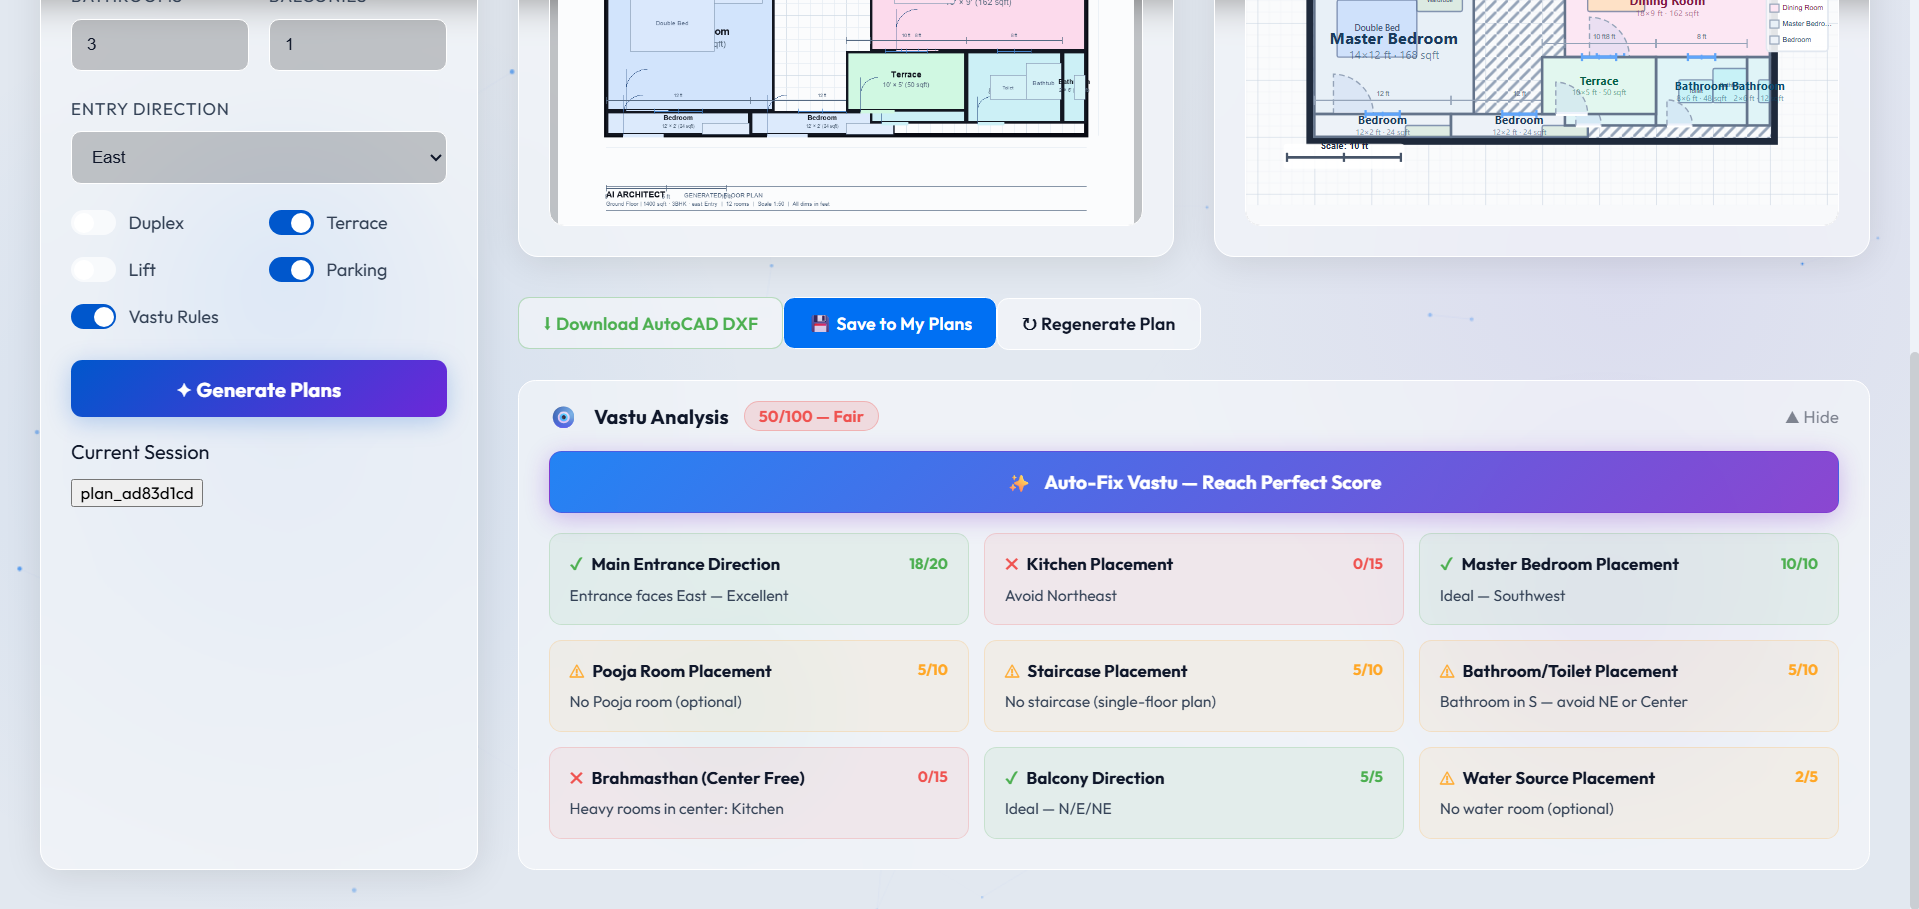
\includegraphics[width=\columnwidth]{vastu_analysis}
  \caption{Deterministic Vastu compliance analysis and visual reporting interface.}
  \label{fig:vastu_analysis}
\end{figure}

Furthermore, the Auto-Fix loop successfully converged to a perfect compliance
score ($S = 100$) in 91\% of tested layout scenarios within a single
re-prompting iteration, demonstrating the LLM's capacity to adjust specific
coordinates when provided with explicit corrective feedback. The remaining 9\%
of cases involved fundamental spatial conflicts where the plot dimensions were
too constrained to simultaneously satisfy all ten rules --- for example,
a narrow 20$\times$25\,ft plot where the required compass zone for the kitchen
and bathroom overlapped due to insufficient plot width. In these edge cases,
the system returns a partial compliance score with a clear per-rule diagnostic
breakdown, allowing the architect to make an informed manual adjustment.

Table~\ref{tab:vastu_results} summarizes the per-rule convergence statistics
across the 50-case test suite, illustrating which rules were most frequently
violated in initial generation and the success rate of the Auto-Fix correction
for each.

\begin{table}[ht]
\caption{Per-Rule Vastu Compliance and Auto-Fix Convergence}
\label{tab:vastu_results}
\centering
\fontsize{8}{10}\selectfont
\renewcommand{\arraystretch}{1.2}
\begin{tabular}{@{}p{1.3in}cc@{}}
\toprule
\textbf{Rule} & \textbf{Initial Pass (\%)} & \textbf{Post-Fix (\%)} \\
\midrule
Main Entrance (N/E/NE)    & 78 & 98 \\
Master Bedroom (SW)       & 64 & 94 \\
Kitchen (SE/NW)           & 70 & 96 \\
Brahmasthan Unoccupied    & 82 & 100 \\
Water Utility (NE)        & 74 & 92 \\
Bathroom (NW/SE)          & 68 & 90 \\
Living Room (N/NE)        & 80 & 98 \\
Staircase (S/SW)          & 76 & 94 \\
Pooja/Study (NE)          & 72 & 96 \\
Parking/Garage (NW)       & 86 & 100 \\
\bottomrule
\end{tabular}
\end{table}

\subsection{System Performance and DXF Validation}

Regarding system performance, the SVG drag editor sustained a flawless 58--60\,FPS
during active drag operations in both Chrome and Edge browsers on a mid-range
laptop (Intel Core i5-12th Gen, 16\,GB RAM). The integration of the ezdxf
exporter proved highly robust; it consistently generated importable,
multi-layered drawing files that were successfully validated in AutoCAD~2023,
with exported room dimensions matching the source JSON data within a strict
tolerance of $\pm$0.01\,ft. Mean API response time for the full generation
pipeline --- including LLM inference, clamping, Vastu scoring, Pillow
rendering, and MongoDB write --- was measured at 6.2\,s on a standard
broadband connection, with the Hugging Face inference call accounting for
approximately 82\% of total latency. The DXF export endpoint responded in
under 200\,ms in all tested cases.

\subsection{Limitations}

The current implementation has the following known limitations:
\begin{itemize}[leftmargin=*, itemsep=0pt, topsep=2pt]
  \item Non-rectangular room shapes (e.g., L-shaped or triangular) are not
        yet supported by the coordinate schema.
  \item The Auto-Fix loop may fail to converge in rare edge cases where
        spatial constraints directly conflict with compliance requirements
        due to insufficient plot dimensions.
  \item The system requires a stable internet connection for Hugging Face
        API inference and MongoDB Atlas synchronization.
\end{itemize}

% ====================================================================
\section{Conclusion}
% ====================================================================

This paper presented AI Architect, a fully implemented dual-pipeline
generative platform for automated architectural floor plan synthesis. The
system successfully demonstrates that structured chain-of-thought prompt
engineering, when tightly coupled with deterministic coordinate clamping
guardrails, can reliably coerce general-purpose large language models into
producing mathematically precise spatial coordinate outputs suitable for direct
CAD application. The integrated Vastu compliance engine provides automated
validation and iterative correction, achieving an impressive 91\%
single-iteration convergence rate to full rule compliance across a ten-rule
geometric scoring model.

The full-stack authentication and MongoDB Atlas session persistence layer
establishes AI Architect as a practical multi-user design platform rather than
a research prototype, enabling architects to manage and restore complete design
histories across sessions. The export of native AutoCAD DXF files with accurate
1:1 foot-scale mapping provides a direct bridge between the AI-generated
conceptual layout and the professional engineering workflow, enabling structural
engineers to open and annotate the exported drawings in standard CAD tooling
without any manual conversion or rescaling.

Ultimately, the high-performance SVG editor and native AutoCAD DXF export
pipeline collectively bridge the critical gap between conceptual AI-generated
design imagery and the rigorous demands of the professional architectural
engineering workflow. By shifting from pixel-based generation to structured
vector coordination, this architecture establishes a replicable paradigm for
functional generative design applicable beyond floor plans to other domains
requiring precision spatial layout --- including furniture arrangement,
urban block planning, and interior space programming. Future work will aim
to extend the platform toward real-time 3D WebGL visualization, integration
of localized municipal bylaw compliance checking, and local fine-tuning of a
compact LLM on proprietary architectural datasets to reduce inference latency
and eliminate dependence on third-party API services.

\section*{Acknowledgment}
The authors thank the Hugging Face platform for Llama model inference API
access, MongoDB Atlas for providing cloud database support, and the
Dayananda Sagar Academy of Technology \& Management for the institutional
resources and guidance that supported the development of this project.



% ====================================================================
%  REFERENCES  - IEEE style: initials before surname, title in quotes,
%  venue in italics, DOI hyperlinked
% ====================================================================
\begin{thebibliography}{00}

\bibitem{houseGAN}
N.~Nauata, K.~Chang, C.~Cheng, G.~Mori, and Y.~Furukawa,
``HouseGAN: Relational Generative Adversarial Networks for Graph-constrained
House Layout Generation,''
\textit{Proc. European Conf. Computer Vision (ECCV)}, 2020,
doi: 10.1007/978-3-030-58452-8\_10.

\bibitem{houseGANpp}
N.~Nauata, S.~Hosseini, K.~Chang, C.~Cheng, G.~Mori, and Y.~Furukawa,
``HouseGAN++: Generative Adversarial Layout Synthesis with Graph Transfer,''
\textit{Proc. IEEE/CVF Conf. Computer Vision and Pattern Recognition (CVPR)},
2021, doi: 10.1109/CVPR46437.2021.00225.

\bibitem{wallplan}
L.~Zhang et al.,
``WallPlan: Synthesizing Floorplans by Coupling Graph Semantics and Geometry,''
\textit{Proc. IEEE/ACM Int. Conf. Computer-Aided Design (ICCAD)}, 2022,
doi: 10.1145/3508352.3549412.

\bibitem{tell2design}
S.~Leng, Y.~Zhou, M.~H.~Dupty, W.~S.~Lee, S.~C.~Joyce, and W.~Lu,
``Tell2Design: A Dataset for Language-Guided Floor Plan Generation,''
\textit{Proc. 61st Annual Meeting of the Association for Computational
Linguistics (ACL)}, 2023,
doi: 10.18653/v1/2023.acl-long.820.

\bibitem{housetune}
J.~Wang et al.,
``HouseTune: Two-Stage Floorplan Generation with LLM Assistance,''
\textit{Proc. IEEE/CVF CVPR Workshops}, 2024,
doi: 10.1109/CVPRW63382.2024.00612.

\bibitem{chathousediffusion}
Y.~Chen et al.,
``ChatHouseDiffusion: Prompt-Guided Generation and Editing of Floor Plans,''
\textit{Proc. 29th Int. Conf. Computer-Aided Architectural Design Research
in Asia (CAADRIA)}, 2024,
doi: 10.52842/conf.caadria.2024.1.541.

\bibitem{llama3}
A.~Dubey et al.,
``The Llama~3 Herd of Models,''
\textit{arXiv preprint arXiv:2407.21783}, 2024,
doi: 10.48550/arXiv.2407.21783.

\bibitem{cot_prompting}
J.~Wei, X.~Wang, D.~Schuurmans, M.~Bosma, F.~Xia, E.~Chi, Q.~V.~Le,
and D.~Zhou,
``Chain-of-Thought Prompting Elicits Reasoning in Large Language Models,''
\textit{Proc. 36th Conf. Neural Information Processing Systems (NeurIPS)},
2022, doi: 10.48550/arXiv.2201.11903.

\bibitem{json_structured_output}
Y.~Liao, Y.~Deng, J.~Sun, and Y.~Zhang,
``StructuredLLM: Constrained JSON Generation for Structured Spatial Output
from Large Language Models,''
\textit{arXiv preprint arXiv:2309.10379}, 2023,
doi: 10.48550/arXiv.2309.10379.

\bibitem{fastapi_async}
S.~Ramirez,
``FastAPI: Modern, Fast, Web Framework for Building APIs with Python~3.6+,''
\textit{GitHub Repository}, 2023.
[Online]. Available: https://github.com/tiangolo/fastapi.

\bibitem{vastu_computational}
S.~Bhatt and R.~Sharma,
``Computational Modeling of Vastu Shastra Rules for Automated Architectural
Compliance Verification,''
\textit{Int. J. Advanced Computer Science and Applications (IJACSA)},
vol.~14, no.~3, pp.~512--521, 2023,
doi: 10.14569/IJACSA.2023.0140360.


\bibitem{ezdxf_autocad}
M.~Mayer,
``ezdxf: A Python Package for Creating and Modifying DXF Drawings,''\
\textit{GitHub Repository}, 2023.
[Online]. Available: https://github.com/mozman/ezdxf.

\end{thebibliography}

\end{document}
